\mbox{$\displaystyle +\,$\,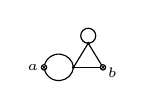
\begin{tikzpicture}[x=0.340cm, y=0.340cm, line width=0.420pt, baseline={([yshift=-0.6ex]0,0)}]
  \draw (-1.100,0.000) arc[start angle=186.026, end angle=353.974, radius=0.553];
  \draw (-1.100,0.000) arc[start angle=173.974, end angle=6.026, radius=0.553];
  \draw (1.100,0.000) -- (0.550,0.900);
  \draw (1.100,0.000) -- (0.000,0.000);
  \draw (0.550,0.900) -- (0.000,0.000);
  \draw (0.550,0.900) arc[start angle=270.000, end angle=630.000, radius=0.280];
  \draw[fill=white] (-1.100,0.000) circle (0.100);
  \draw[line width=0.298pt] (-1.030,0.070) -- (-1.170,-0.070) (-1.030,-0.070) -- (-1.170,0.070);
  \draw[fill=white] (1.100,0.000) circle (0.100);
  \draw[line width=0.298pt] (1.170,0.070) -- (1.030,-0.070) (1.170,-0.070) -- (1.030,0.070);
  \fill (0.550,0.900) circle (0.064);
  \fill (0.000,0.000) circle (0.064);
  \node[font=\tiny, inner sep=0pt, anchor=0] at (-1.290,0.000) {$a$};
  \node[font=\tiny, inner sep=0pt, anchor=151] at (1.266,-0.093) {$b$};
\end{tikzpicture}}
\diagramgap
\mbox{$\displaystyle +\,$\,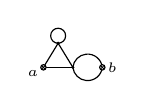
\begin{tikzpicture}[x=0.340cm, y=0.340cm, line width=0.420pt, baseline={([yshift=-0.6ex]0,0)}]
  \draw (-1.100,0.000) -- (-0.550,0.900);
  \draw (-1.100,0.000) -- (0.000,0.000);
  \draw (1.100,0.000) arc[start angle=353.974, end angle=186.026, radius=0.553];
  \draw (1.100,0.000) arc[start angle=6.026, end angle=173.974, radius=0.553];
  \draw (-0.550,0.900) -- (0.000,0.000);
  \draw (-0.550,0.900) arc[start angle=270.000, end angle=630.000, radius=0.280];
  \draw[fill=white] (-1.100,0.000) circle (0.100);
  \draw[line width=0.298pt] (-1.030,0.070) -- (-1.170,-0.070) (-1.030,-0.070) -- (-1.170,0.070);
  \draw[fill=white] (1.100,0.000) circle (0.100);
  \draw[line width=0.298pt] (1.170,0.070) -- (1.030,-0.070) (1.170,-0.070) -- (1.030,0.070);
  \fill (-0.550,0.900) circle (0.064);
  \fill (0.000,0.000) circle (0.064);
  \node[font=\tiny, inner sep=0pt, anchor=29] at (-1.266,-0.093) {$a$};
  \node[font=\tiny, inner sep=0pt, anchor=180] at (1.290,0.000) {$b$};
\end{tikzpicture}}
\diagramgap
\mbox{$\displaystyle +\,$\,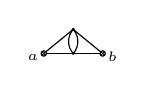
\begin{tikzpicture}[x=0.340cm, y=0.340cm, line width=0.420pt, baseline={([yshift=-0.6ex]0,0)}]
  \draw (-1.100,0.000) -- (0.000,0.000);
  \draw (-1.100,0.000) -- (0.000,0.900);
  \draw (1.100,0.000) -- (0.000,0.000);
  \draw (1.100,0.000) -- (0.000,0.900);
  \draw (0.000,0.000) arc[start angle=317.884, end angle=402.116, radius=0.671];
  \draw (0.000,0.000) arc[start angle=222.116, end angle=137.884, radius=0.671];
  \draw[fill=white] (-1.100,0.000) circle (0.100);
  \draw[line width=0.298pt] (-1.030,0.070) -- (-1.170,-0.070) (-1.030,-0.070) -- (-1.170,0.070);
  \draw[fill=white] (1.100,0.000) circle (0.100);
  \draw[line width=0.298pt] (1.170,0.070) -- (1.030,-0.070) (1.170,-0.070) -- (1.030,0.070);
  \fill (0.000,0.000) circle (0.064);
  \fill (0.000,0.900) circle (0.064);
  \node[font=\tiny, inner sep=0pt, anchor=20] at (-1.279,-0.064) {$a$};
  \node[font=\tiny, inner sep=0pt, anchor=160] at (1.279,-0.064) {$b$};
\end{tikzpicture}}
\diagramgap
\mbox{$\displaystyle +\,\frac{1}{2}$\,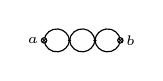
\begin{tikzpicture}[x=0.340cm, y=0.340cm, line width=0.420pt, baseline={([yshift=-0.6ex]0,0)}]
  \draw (-1.425,0.000) arc[start angle=186.026, end angle=353.974, radius=0.478];
  \draw (-1.425,0.000) arc[start angle=173.974, end angle=6.026, radius=0.478];
  \draw (1.425,0.000) arc[start angle=353.974, end angle=186.026, radius=0.478];
  \draw (1.425,0.000) arc[start angle=6.026, end angle=173.974, radius=0.478];
  \draw (-0.475,0.000) arc[start angle=186.026, end angle=353.974, radius=0.478];
  \draw (-0.475,0.000) arc[start angle=173.974, end angle=6.026, radius=0.478];
  \draw[fill=white] (-1.425,0.000) circle (0.100);
  \draw[line width=0.298pt] (-1.355,0.070) -- (-1.495,-0.070) (-1.355,-0.070) -- (-1.495,0.070);
  \draw[fill=white] (1.425,0.000) circle (0.100);
  \draw[line width=0.298pt] (1.495,0.070) -- (1.355,-0.070) (1.495,-0.070) -- (1.355,0.070);
  \fill (-0.475,0.000) circle (0.064);
  \fill (0.475,0.000) circle (0.064);
  \node[font=\tiny, inner sep=0pt, anchor=0] at (-1.615,0.000) {$a$};
  \node[font=\tiny, inner sep=0pt, anchor=180] at (1.615,0.000) {$b$};
\end{tikzpicture}}
\diagramgap
\mbox{$\displaystyle +\,$\,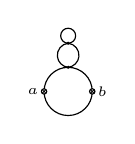
\begin{tikzpicture}[x=0.340cm, y=0.340cm, line width=0.420pt, baseline={([yshift=-0.6ex]0,0)}]
  \draw (-0.900,0.000) arc[start angle=180.000, end angle=360.000, radius=0.900];
  \draw (-0.900,0.000) arc[start angle=180.000, end angle=90.000, radius=0.900];
  \draw (0.900,0.000) arc[start angle=0.000, end angle=90.000, radius=0.900];
  \draw (0.000,1.800) arc[start angle=96.026, end angle=263.974, radius=0.452];
  \draw (0.000,1.800) arc[start angle=83.974, end angle=-83.974, radius=0.452];
  \draw (0.000,1.800) arc[start angle=270.000, end angle=630.000, radius=0.280];
  \draw[fill=white] (-0.900,0.000) circle (0.100);
  \draw[line width=0.298pt] (-0.830,0.070) -- (-0.970,-0.070) (-0.830,-0.070) -- (-0.970,0.070);
  \draw[fill=white] (0.900,0.000) circle (0.100);
  \draw[line width=0.298pt] (0.970,0.070) -- (0.830,-0.070) (0.970,-0.070) -- (0.830,0.070);
  \fill (0.000,1.800) circle (0.064);
  \fill (0.000,0.900) circle (0.064);
  \node[font=\tiny, inner sep=0pt, anchor=0] at (-1.090,-0.001) {$a$};
  \node[font=\tiny, inner sep=0pt, anchor=180] at (1.090,-0.001) {$b$};
\end{tikzpicture}}
\diagramgap
\mbox{$\displaystyle +\,\frac{2}{3}$\,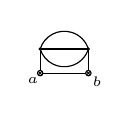
\begin{tikzpicture}[x=0.340cm, y=0.340cm, line width=0.420pt, baseline={([yshift=-0.6ex]0,0)}]
  \draw (-0.900,0.000) -- (0.900,0.000);
  \draw (-0.900,0.000) -- (-0.900,0.900);
  \draw (0.900,0.000) -- (0.900,0.900);
  \draw (-0.900,0.900) arc[start angle=197.189, end angle=342.811, radius=0.942];
  \draw (-0.900,0.900) -- (0.900,0.900);
  \draw (-0.900,0.900) arc[start angle=162.811, end angle=17.189, radius=0.942];
  \draw[fill=white] (-0.900,0.000) circle (0.100);
  \draw[line width=0.298pt] (-0.830,0.070) -- (-0.970,-0.070) (-0.830,-0.070) -- (-0.970,0.070);
  \draw[fill=white] (0.900,0.000) circle (0.100);
  \draw[line width=0.298pt] (0.970,0.070) -- (0.830,-0.070) (0.970,-0.070) -- (0.830,0.070);
  \fill (-0.900,0.900) circle (0.064);
  \fill (0.900,0.900) circle (0.064);
  \node[font=\tiny, inner sep=0pt, anchor=45] at (-1.034,-0.134) {$a$};
  \node[font=\tiny, inner sep=0pt, anchor=135] at (1.034,-0.134) {$b$};
\end{tikzpicture}}
\diagramgap
\mbox{$\displaystyle +\,\frac{1}{2}$\,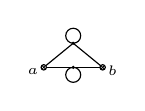
\begin{tikzpicture}[x=0.340cm, y=0.340cm, line width=0.420pt, baseline={([yshift=-0.6ex]0,0)}]
  \draw (-1.100,0.000) -- (0.000,0.000);
  \draw (-1.100,0.000) -- (0.000,0.900);
  \draw (1.100,0.000) -- (0.000,0.000);
  \draw (1.100,0.000) -- (0.000,0.900);
  \draw (0.000,0.000) arc[start angle=90.000, end angle=450.000, radius=0.280];
  \draw (0.000,0.900) arc[start angle=270.000, end angle=630.000, radius=0.280];
  \draw[fill=white] (-1.100,0.000) circle (0.100);
  \draw[line width=0.298pt] (-1.030,0.070) -- (-1.170,-0.070) (-1.030,-0.070) -- (-1.170,0.070);
  \draw[fill=white] (1.100,0.000) circle (0.100);
  \draw[line width=0.298pt] (1.170,0.070) -- (1.030,-0.070) (1.170,-0.070) -- (1.030,0.070);
  \fill (0.000,0.000) circle (0.064);
  \fill (0.000,0.900) circle (0.064);
  \node[font=\tiny, inner sep=0pt, anchor=20] at (-1.279,-0.064) {$a$};
  \node[font=\tiny, inner sep=0pt, anchor=160] at (1.279,-0.064) {$b$};
\end{tikzpicture}}
\diagramgap
\mbox{$\displaystyle +\,$\,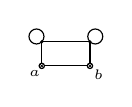
\begin{tikzpicture}[x=0.340cm, y=0.340cm, line width=0.420pt, baseline={([yshift=-0.6ex]0,0)}]
  \draw (-0.900,0.000) -- (0.900,0.000);
  \draw (-0.900,0.000) -- (-0.900,0.900);
  \draw (0.900,0.000) -- (0.900,0.900);
  \draw (-0.900,0.900) -- (0.900,0.900);
  \draw (-0.900,0.900) arc[start angle=315.000, end angle=675.000, radius=0.280];
  \draw (0.900,0.900) arc[start angle=225.000, end angle=585.000, radius=0.280];
  \draw[fill=white] (-0.900,0.000) circle (0.100);
  \draw[line width=0.298pt] (-0.830,0.070) -- (-0.970,-0.070) (-0.830,-0.070) -- (-0.970,0.070);
  \draw[fill=white] (0.900,0.000) circle (0.100);
  \draw[line width=0.298pt] (0.970,0.070) -- (0.830,-0.070) (0.970,-0.070) -- (0.830,0.070);
  \fill (-0.900,0.900) circle (0.064);
  \fill (0.900,0.900) circle (0.064);
  \node[font=\tiny, inner sep=0pt, anchor=45] at (-1.034,-0.134) {$a$};
  \node[font=\tiny, inner sep=0pt, anchor=135] at (1.034,-0.134) {$b$};
\end{tikzpicture}}
